\documentclass[ngerman]{scrartcl}

\usepackage[utf8]{inputenc}
\usepackage{babel}
\usepackage[T1]{fontenc}
\usepackage{lmodern}
\usepackage{color}
\usepackage{graphicx}
\usepackage[colorlinks=true, linkcolor=cyan]{hyperref}
\usepackage{enumerate}
\usepackage{amsmath}
\usepackage{braket}
\newcommand{\erw}[1]{\langle {#1} \rangle}
\newcommand{\Hil}{\mathcal{H}}
\newcommand{\diff}{\mathrm{d}}

\usepackage[backend=bibtex, style=numeric-comp, sorting=nty]{biblatex}
\bibliography{mybib}

%\usepackage{scrpage2}
%\usepackage{booktabs}
%\usepackage{cite}
%\usepackage{makeidx}
%\makeindex
%\pagestyle{scrheadings}
\begin{document}
 
	\begin{titlepage}
		\begin{minipage}[c][\textheight][c]{\textwidth}
			\begin{center}
				{ \Huge \textbf{Thermodynamik schwarzer Löcher} }
				
				\vspace*{1cm}
				{\large eine Seminararbeit von}
				
				\vspace*{0.2cm}
				{\Large Tamara Szecsey}
				
				\vspace*{1cm}
				{\large \today}
				
				\vspace*{4cm}
				\hspace*{1cm} 
\includegraphics[height=30ex]{LOGO_UR}
			\end{center}
		\end{minipage}
	\end{titlepage}
	
\tableofcontents
\newpage

\section{Informationsentropie im Allgemeinen} \label{InfoentropieAllg}
Zunächst ein kurzer Einblick, um welche Art von Entropie es sich hier handeln wird. Ludwig Boltzmann hatte festgestellt, dass eine Proportionalität zwischen der Entropie $S$ und $\log W$ herrscht, wobei $W$ die Wahrscheinlichkeit darstellt. Der zugehörige Proportionalitätsfaktor $k$ ist die Boltzmann-Konstante.
	\begin{align}
		S &= k \log W
	\end{align}
Dies ist eine wichtige Verbindung zwischen Statistik und Thermodynamik. 
Die Verallgemeinerte Boltzmannsche Beziehung bring dann die sogenannte Informationsentropie hervor, die in diesen Gestalten geschrieben werden kann:	
	\begin{align} \label{Informationsentropie}
		S &=
		\left\{
		\begin{aligned}
		&- k ~\erw{\,\ln \rho\,} \\
		&-k~ Sp(\rho \ln \rho) \\
		&-k \sum_n \rho_n \ln \rho_n
		\end{aligned}
		\right.
	\end{align}
wobei $\rho$ die Wahrscheinlichkeit ist, die Energie $E_n$ im mikrokanonischen Ensemble anzutreffen. 
(Wir wollen hier nicht weiter auf die thermodynamische Definition der Entropie eingehen, für Fragen zu den Grundlagen siehe \cite{Brenig})

Wie wir jetzt aber zu Information kommen, soll ein Beispiel zeigen. Dabei geht es um eine quantitativen Betrachtung der selben.
Wir betrachten nun eine Reihe von Ereignissen $E_n (n = 1, 2, \ldots, N)$, die mit bestimmten Wahrscheinlichkeiten $\rho_n$ auftreten, wobei
	\begin{align}
		\sum_{n=1}^N \rho_n &= 1
	\end{align}
Nun sehen wir das Eintreten bestimmter die Ereignisse $E_n$, dabei hat jede unserer Feststellungen hat einen Informationswert $I_n$. Nach häufiger Wiederholung kann man einen mittleren Informationsgehalt aufstellen:
	\begin{align}
		I = \sum_{n=1}^N
	\end{align}
Hier legen wir wie in der Informationstheorie fest
	\begin{align} \label{Informationsgehalt}
		I = - \sum \rho_n \mathrm{ld}(\rho_n)
	\end{align}
wobei $\mathrm{ld}(x)$ der dyadische Logarithmus von $x$ ist, also $2^{\mathrm{ld}(x)} = x$. 
Wir haben \eqref{Informationsgehalt} so festgelegt, dass ein Ereignis allein durch eine Ja oder Nein Frage (oder durch 0 und 1) vollständig charakterisierbar ist. 
Dass unserer mittlerer Informationsgehalt unserer Entropie von \eqref{Informationsentropie} ähnlich sieht, ist kein Zufall.

Wir machen nun zwei Zahlenbeispiele zur Veranschaulichung:
	\begin{itemize}
		\item[\textit{1.\,Beispiel:}] Sei $N=2, \rho_1 = \rho_2= \frac{1}{2}$ was sein könnte: Ein Teilchen hält sich mit gleicher Wahrscheinlichkeit in der linken oder rechten Hälfe eines Kastens auf, oder Zahl und Wappen für ein Münzwurf.
		Es benötigt Ja-Nein-Frage, um herauszufinden, wo das Teilchen liegt oder wie herum die Münze gefallen ist.
			\begin{align}
				I = \mathrm{ld}(2) = 1 \,\mathrm{bit}
			\end{align}
		Ein bit ist die Einheit für Information.
		\item[\textit{2.\,Beispiel:}]Sei $N=6, \rho_n = \frac{1}{6}$, wobei die Ereignisse $E_n$ die Seiten eines Würfels sein könnten, der Informationsgehalt
			\begin{align}
				I = \mathrm{ld}(6) &= 2,58 \,\mathrm{bit}
			\end{align}
	\end{itemize}
(siehe auch \cite{Brenig})

\section{In Verbindung mit Verschränkungsentropie (Entanglement Entropy)} %S.87
	Von einer Verschränkung spricht man bei Korrelationen zwischen zwei Untersystemen. Wir brauchen sie später für die Informationsentropie.
		
	Es seien zwei Untersysteme $A$ und $B$, das Untersystem $A(B)$ wird beschrieben durch ein komplette Menge an kommutierenden Opservablen $\alpha(\beta)$. Die Zusammensetzung beider Systeme wäre in einem reinen Zustand (falls das unbekannt ist, siehe Anhang \ref{ReinerZustandA}) durch die Wellenfunktion $\Psi(\alpha,\beta)$ beschrieben. Sie sind zunächst separiert voneinander, alle Messungen die an $A(B)$ gemacht werden, können mit Hilfe der Dichtematrix $\rho_A(\rho_B)$ beschrieben werden.
	
	Also für ein $\alpha'$ welches in $\alpha$ übergeht und ein $\beta'$ welches in ein $\beta$ übergeht bedeutet das:
		\begin{align}
			\begin{aligned}
			(\rho_A)_{\alpha \alpha'} &=
			\sum_{\beta} \Psi^*(\alpha, \beta) \Psi(\alpha', \beta) \\
			(\rho_B)_{\beta \beta'} &= 
			\sum_{\alpha} \Psi^* (\alpha, \beta) \Psi (\alpha, \beta')
			\end{aligned}
		\end{align}
	Wir gehen nun von $\rho_A$ aus, um die Eigenschaften der Dichtematrix zu betrachten (wir könnten auch problemlos von $\rho_B$ ausgehen)
	\begin{enumerate}[1)]
		\item Die Dichtematrix ist hermitesch
			\begin{align}
				(\rho_A)_{\alpha \alpha'} &= (\rho_A)^*_{\alpha' \alpha}
			\end{align}
		\item Die Dichtematrix ist positiv semidefinit, also alle ihre Eigenwerte sind 0 oder positiv.
		\item Die Dichtematrix ist auf 1 normalisiert:
			\begin{align}
				Sp \, \rho = 1
			\end{align}
		Das bedeutet nun aber, dass die Eigenwerte nur Zahlen zwischen eins und null annehmen können. Wenn ein Eigenwert von $\rho_A$ gleich 1 ist, dann müssen alle Anderen verschwinden, und in dem Falle wäre dann $A$ in einem reinen Zustand. 
		Dies geschieht nur, wenn die Wellenfunktion sich wie folgt faktorisieren lässt:
			\begin{align}
				\Psi (\alpha, \beta) &= \psi_A(\alpha) \psi_B (\beta)
			\end{align} 
		(hier wäre auch $B$ in einem reinen Zustand)
		\item Die nicht-verschwindenden Eigenwerte von $\rho_A$ und $\rho_B$ sind gleich, wenn das Verbundsystem in einem reinen Zustand ist. (Ein Beweis ist zu finden auf S.72 \cite{Revolution})
	\end{enumerate}
Aus Letzterem folgt folgendes für Verschränkungsentropie:
	\begin{align}
		S_A = -Sp \, \rho_A \log \rho_A = S_B
	\end{align}
Und in dem Fall ist die Entropie des kombinierten Systems $S_{A+B} = 0$.

Nun betrachten wir ein großes System $\Sigma$, welches in viele kleine, gleiche Untersysteme $\sigma_i$. Wir nehmen an, dass diese Untersysteme schwach miteinander wechselwirken und das ganze System sich in einem reinen Zustand mit Gesamtenergie $E$ befindet, wobei die Untersysteme im Durchschnitt eine Energie $\epsilon$ besitzen. Die Entropie des Gesamtsystems soll verschwindend sein.

Die kleinen Untersysteme haben wie aus der Thermodynamik bekannt eine Dichtematrix
	\begin{align}
		\rho_i = \frac{e^{-\beta H_i}}{Z_i}
	\end{align}	
($H_i$ Energy des Untersystems)

Diese maximiert die Entropie für eine gegebene, mittlere Energie $\epsilon$.
Die \textit{grob körnig} (oder auch \textit{Thermalentropie} genannt) des Verbundsystems ist definiert, als die Summe der Entropien aller Untersysteme
	\begin{align}
		S_{\text{Thermal}} = \sum_i S_i 
	\end{align}
Diese ist nicht erhalten und wir kennen sie aus thermodynamischem Kontext.

Nun interagieren die Untersysteme miteinander. Da die Wellenfunktion dadurch nicht mehr faktorisiert werden kann, sind alle Entropien der Untersysteme nicht null ($S_i \neq 0$)
und die \textit{grob körnige} Entropie auch
	\begin{align*}
		S_{\text{Thermal}} = \sum_i S_i \neq 0
	\end{align*}
Wir definieren noch eine \textit{fein körnige} Entropie eines Untersystems $\Sigma_1$ von $\Sigma$ welches eine Verschränkungsentropie $S(\Sigma_1)$ von $\Sigma_1$ mit einem übrigbleibenden Untersystem $\Sigma-\Sigma_1$ ist.  

In unserem obigen Fall wäre die \textit{fein körnige} Entropie von $\Sigma$ erhalten und gleich null. 

Außerdem wird immer gelten:
	\begin{align}
		S_{\text{Thermal}}(\Sigma_1) > S(\Sigma_1)
	\end{align}
Das bedeutet, die grob körnige Entropie wird immer größer als die fein Körnige sein.

Nun können wir die Information definieren als.
	\begin{align}
		I = S_{\text{Thermal}} - S
	\end{align}
Wenn die grob körnige Entropie die Thermalentropie eines Systems ist, wie häufig der Fall, dann ist die Information die Differenz zwischen dieser und der feinkörnigen, also der Verschränkungsentropie.

In einem kleinen Untersystem verschwindet die Information, genauso wie in einem kombinierten System $\Sigma$ die Information maximal wird, da die gesamte Thermalentropie vorhanden ist.

Was passiert aber in einem mittelgroßen Untersystem? Statt der Erwartung, dass die Information stetig von 0 (für $\sigma_i$) zu $S_{\text{Thermal}}$ (für $\Sigma$) wandert, wird sie für alle Untersysteme kleiner als $\frac{1}{2}$ vom ganzen System verschwindend gering. 

Dass Information in bit mit einem numerischen Wert $\log 2$ gerechnet wird, wissen wir seit Kap. \ref{InfoentropieAllg}. Für ein typisches Untersystem, welches kleiner als die Hälfte von $\Sigma$ ist, ist die Information kleiner als 1 bit, bei genau der Hälfte beträgt sie ungefähr 1 bit. In anderen Worten für $\Sigma_1 < \frac{1}{2} \Sigma$ 
	\begin{align*}
		S(\Sigma_1) &\cong S_{\text{Thermal}}(\Sigma_1) \\
		I(\Sigma_1) &\approx 0
	\end{align*}
Als nächstes betrachten wir ein System mit $\Sigma_1 > \frac{1}{2} \Sigma$. Wir benutzen
	\begin{align}
		\left.
		\begin{aligned}
			S(\Sigma - \Sigma_1) &= S(\Sigma_1) \\
			S(\Sigma - \Sigma_1) &\cong S_{\text{Thermal}} (\Sigma - \Sigma_1)
		\end{aligned}
		\right\}
		\Rightarrow S(\Sigma_1) = S_{\text{Thermal}} (\Sigma - \Sigma_1)
	\end{align}
Die grobe Entropie von $\Sigma - \Sigma_1$ wird in der Ordnung $(1- f) S_{\text{Thermal}}(\Sigma)$ sein, wobei $f$ der Anteil aller einfacher Freiheitsgrade\footnote{Ein einzelner einfacher Freiheitsgrad repräsentiert ein einzelnen Bit an Information. Mit einem Freiheitsgrad ist soetwas wie ein Spin oder die An- bzw. Abwesenheit eines Fermions gemeint.} ist, die in $\Sigma_1$ vorkommen. 

Die Information ist nun
	\begin{align}
		\begin{aligned}
		I (\Sigma_1) &= S_{\text{Thermal}}(\Sigma_1) - S(\Sigma_1) \\
		&= f\, S_{\text{Thermal}} (\Sigma) - (1 - f)S_{\text{Thermal}}(\Sigma) \\
		&= (2f - 1) S_{\text{Thermal}}(\Sigma) 
		\end{aligned}
	\end{align}

Um später auf die Verdunstung schwarzer Löcher und deren Information zurückzukommen, werden wir jetzt erstmal ein Gedankenexperiment machen, in der noch die bekannten Gesetze der Physik gelten.

Wir stellen uns eine Box mit Wenden an denen alles reflektiert wird. Innerhalb liegt eine Bombe die explodieren kann. Außerdem hat sie noch ein sehr kleines Loch, aus dem Strahlung entweichen kann.
Das gesamte System $\Sigma$ ist aufgeteilt in das innere Untersystem $B$ und in das gesamte Äußere $A$ der Box. 

Anfangs ist die Bombe im Grundzustand und die Entropie von $B$ ist verschwindend gering.
Sobald die Bombe hoch geht setzt sie thermische Strahlung frei, welche die Box füllt. Die feinkörnige Entropie ändert sich nicht, aber die thermische Entropie steigt. Da noch kein Photon entweichen konnte, ändert sich auch nicht an der äußeren Entropie.
	\begin{align}
		\begin{aligned}
			S_{\text{Thermal}} (B) &\neq 0 \\
			S(B) = 0 &~~~ S(A) = 0
		\end{aligned}
	\end{align}
Als nächstes werden die Photonen langsam hinaus strömen mit dem Ergebnis, dass das Innere und Äußere der Box verschränken. Die Verschränkungsentropie ($A$ und $B$ haben die Selbe) steigt, während die thermische Entropie sinkt. 
	\begin{align}
	\begin{aligned}
	S_{\text{Verschränkung}} &\neq 0 \\
	S_{\text{Thermal}} (B) \neq 0 &~~~ S_{\text{Thermal}}(A) \neq 0
	\end{aligned}
	\end{align}
Wenn alle Photonen die Box verlassen, dann wird sie wieder im Grundzustand sein und die verschiedenen Entropien werden zurück auf null gehen.
	
	BILD AUF SEITE 92 EINFÜGEN BITTE

\section{Das holographische Prinzip}
Wir befinden uns in der String Theorie in einem flachen Raum. Wir schauen nun auf eine Region $\Gamma$ in so Einem. 

Die maximale Entropie aller physikalischen Systeme, die in $\Gamma$ hinein passen, sind proportional zur Fläche des Rands $\partial \Gamma$, welche in Planck Einheiten aufgeteilt ist. 

Typischerweise, bei einem Gitter aus Spins, misst die Maximalentropie die einfachen Freiheitsgrade, also wie oben erwähnt so etwas wie den Spin oder Fermionen. Außer in der Gravitationssystemen ist dies proportional zum Volumen $\Gamma$. 

Diese obere Grenze der Entropie sagt uns, dass die maximale Anzahl der sich unterscheidenden Freiheitsgrade proportional zur Fläche ist. Das bedeutet allerdings für große makroskopische Regionen eine enorme Verminderung die Freiheitsgrade. Bei einer Dimension $L$ skaliert die Anzahl der Freiheitsgrade pro Volumen mit $\frac{1}{L}$ in Planck Einheiten.
Wenn wir $L$ groß genug machen, werden die Freiheitsgrade also sehr dünn besiedelt im Raum verteilt sein. Allerdings wollen wir immer noch alle mikroskopischen Prozesse erfassen, die irgendwo in der Region passieren. 

Eine Art und Weise dies zu betrachten ist mit Freiheitsgraden von $\Gamma$, welche alle auf $\partial \Gamma$ leben, mit einer Dichte nicht größer als $\sim 1$ Freiheitsgrad pro Planckfläche. In anderen Worten, wir beschreiben einen dreidimensionalen Raum, nämlich die Kugel um das schwarze Loch mit dem Horizontradius durch ein zweidimensionales Hologramm an der Grenze! Dies nennt man Holographisches Prinzip. 

	\begin{figure}
		\begin{center}
			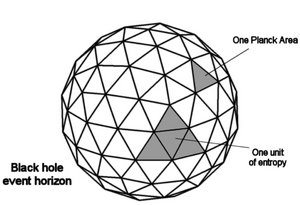
\includegraphics[width=0.6\textwidth]{BHentropy1}
		\end{center}
		\caption{Zweidimensionale Oberfläche des Horizonts aufgeteilt in Planck Einheiten. Die Entropie hat allerdings eine Einheit von 4 solchen Planckflächen für ein Bit. Siehe \ref{BHEntropie}. (aus )}
	\end{figure} 
	%\cite{BekensteinHawking}

\section{Evaporation}
Stephen Hawking hat in seinem Paper \cite{ParticleCreation} gezeigt, dass ein großes schwarzes Loch für einen Beobachter in großer Ferne eine Temperatur besitzt:
\begin{align}
T = \frac{1}{8 \pi MG}
\end{align}


\section{Die Bekenstein-Hawking Entropie} \label{BHEntropie}
Zunächst betrachten wir Gründe, warum ein schwarzes Loch Entropie besitzen muss. 
	\begin{itemize}
		\item Zum einen Form es sich normalerweise durch kollabierende Materie, die eine 	bestimmte Masse haben oder Strahlung abgeben. Beide enthalten 		Entropie. Wir können nach der Entstehung des schwarzen Lochs nicht mehr über den Horizont hinweg sehen, also können wir keine thermodynamische Aussage auf Grundlage der zuvor kollabierten Materie machen, weil sie unbeobachtbar ist. Aber mit einer dem schwarzen Loch zugeordneten Entropie ist das möglich.
		
		\item Ein schwarzes Loch kann mich ein paar wenigen Parametern beschrieben werden, nämlich Masse, elektrische Ladung und Drehmoment. Da für eine beliebige Wahl dieser Zahlen eine Menge Möglichkeiten bestehen, wie das Schwarze Loch entstanden sein könnte, stimmen viele inneren Zustände mit ihm überein. Das passt auch zur Thermodynamik, in der viele Mikrozustände einen Makrozustand bilden können. Genau diesen weiß die Entropie zu beschreiben, deshalb muss ein schwarzes Loch diese haben. 
		
		\item Das Schwarze Loch blockt alle Signale und verhindert somit, dass keine Information über es an die Außenwelt gelangen kann. So gesehen kann man sagen, dass es Information versteckt, die aber durch die Entropie gemessen werden kann. Deshalb macht es Sinn dem schwarzen Loch eine Entropie zuzuschreiben. 
	\end{itemize}
	
	\subsection*{Die Entropie des schwarzen Lochs in Formeln}
	Masse, elektrische Ladung und Drehmoment sind in der gleichen Kombination immer proportional zur Oberfläche des schwarzen Lochs. Sowohl Hawking also auch Misner, Thorne und Wheeler haben gezeigt, dass sein Ereignishorizont nicht kleiner werden kann, meistens wird er sogar größer.
	
	Diese Oberfläche verhält sich sozusagen wie die thermodynamische Entropie in geschlossenen Systemen. 
	Durch die Hawkingtemperatur \cite{ParticleCreation} und der Definition von Temperatur in der Thermodynamik
		\begin{align}
			\frac{\diff S}{\diff E} &= \frac{1}{T},&
			T_{\text{Hawking}} &= \frac{\hbar c^3}{8 \pi G M}
		\end{align}
	und durch ersetzen von $E = Mc^2$, erhalten wir
		\begin{align} \label{SHentropie}
			S_{BH} &= \frac{c^3 A}{4 G \hbar} = \frac{A}{4 L_P^2} 
		\end{align}
	Der Horizont ist an Fläche $A$, welche eine Kugeloberfläche um das schwarze Loch mit dem Schwarzschildradius bildet:
		\begin{align}
			r_h &= \frac{2 GM}{c^2} ,& A = 4 \pi r_h^2 
		\end{align}
	Ein sonnen-schweres schwarzes Loch hätte eine Horizontfläche $\frac{1}{5}$-mal so groß wie die Erdoberfläche und ihre Entropie wäre von der Ordnung $10^{77}$. Dies ist über zehn Größenordnungen höher, als die Entropie der jetzigen Sonne.  
	
	Es scheint also, dass die Entropie des schwarzen Lochs nicht mit der hineingefallenen Entropie während seiner Entstehung verglichen werden kann.
	
	\subsection*{Was wir durch diese Entropie gewinnen}
	Nun folgen ein paar Interpretationen der Entropie der schwarzen Löcher:
	
	\begin{itemize}
		\item [~] \textit{Die Entropie eine schwarzen Lochs zählt die inneren Zustände der Masse und Gravitation.}
	\end{itemize}
	Wie zuvor bereits erwähnt, gibt es viele Möglichkeiten, wie ein bestimmtes schwarze Loch mit fester Masse, Ladung und Drehmoment entstanden ist. Die Zustände der Materie werden den Mikrozuständen dargestellt. Für genauere Beisiele siehe \cite{FrolovNovikov}.
	
	\begin{itemize}
		\item [~] \textit{Die Entropie des schwarzen Lochs ist die Entropie der Verschränkung zwischen Freiheitsgraden innerhalb und außerhalb des Horizonts.}
	\end{itemize}
	Die Freiheitsgrade des Quantenfeldes außerhalb eines schwarzen Lochs, welches bei einem Kollaps entstanden ist, müsste eigentlich mit den Inneren verschränkt sein. Letzteres ist für den Beobachter leider unsichtbar. Jegliche Information hinter dem Horizont über die Freiheitsgrade ist verschwunden, deshalb kann könnte man einen Mischzustand messen, auch wenn er ursprünglich rein war. Aber dieser ist verbunden mit einer Verschränkungsentropie, die wie von Bombelli usw \cite{BombelliKouLeeSorkin} und Srednicki \cite{Srednicki} gezeigt, proportional zur Horizontenfläche ist.
	
	\begin{itemize}
		\item [~] \textit{Die Entropie des schwarzen Lochs zählt die Gravitationszustände am Horizont.}
	\end{itemize}
	Es wurde vorgeschlagen, dass die gesuchten Zustände Gravitationsfreiheitsgrade sind, die sich am Horizont des schwarzen Lochs ansiedeln. Ein Beispiel für diesen Ansatz machte Carlip \cite{Carlip}, wo er auch Gleichung \eqref{SHentropie} herleitet.
	
	\begin{itemize} 
		\item [~] \textit{Die Entropie des schwarzen Lochs ist eine erhaltene Größe verbunden mit Koordinateninvarianz der Gravitationswirkung.}
	\end{itemize}
	Diese Näherung ist von Wald \cite{Wald} gemacht worden. Dieser sagt aus, dass die Entropie schwarzer Löcher Noetherladung der Diffeomorphismus Symmetrie ist.  Hieraus kann man wieder Gleichung \eqref{SHentropie} ableiten, wenn die Gravitationswirkung in erster Ordnung der Krümmung vorliegt. 
	
	\begin{itemize}
		\item [~] \textit{Die Entropie des schwarzen Lochs ist die thermische Entropie der Quanten, welche die thermische Atmosphere des schwarzen Lochs formen.}
	\end{itemize}
	\cite{ThorneZurek} \cite{Hooft}
	
	\begin{itemize}
		\item [~] \textit{Die Entropie des schwarzen Lochs zählt die Zustände oder Anregungen eines fundamentalen String.}
	\end{itemize}
	\cite{BowickSmolinWijewardhana} \cite{Susskind} \cite{StromingerWafa}
	
	\begin{itemize}
		\item [~] \textit{Die Entropie des schwarzen Lochs ist äquivalent zur thermischen Entropie der an der Grenze der Raumzeit zum s1chwarzen Loch angesiedelten Strahlung.}
	\end{itemize}
	\cite{Witten}
	
\section{Wirkungsintegrale}

\section{Loop Quantum Gravity (LQG)}	
Die Loop-Quantengravitation (Loop = Schleifen) ist eine Konkurrenztheorie der Stringtheorie und geht nimmt keine Singularität in der Mitte des schwarzen Lochs an, sondern beinhaltet die Theorie, dass es weiße Löcher gibt, die wie schwarze Löcher, welche rückwärts in der Zeit leben, aussehen. 

\appendix
\section{Reiner Zustand} \label{ReinerZustandA}
Sei $\rho$ die \textit{Dichtematrix} welche ein Quantenzustand im Hilbertraum ist $\Hil$. Quantenzustände werden allgemein mit Operatoren dargestellt, hier: $\rho$ ist ein nicht negativer, hermitescher Operator mit Spur 1. Wenn es in der Form
	\begin{equation}
		\rho=\ket{\psi} \bra{\psi}
	\end{equation}
geschrieben werden kann, dann heißt er \textit{rein}. Wenn ein Zustand nicht rein ist, dann ist er \textit{gemischt}.

\section{Zustände in der Thermodynamik}

\subsection*{Mikrozustand}
Ein Mikrozustand ist im klassischen Fall ein Punkt im Phasenraum. Damit ist Ort und Impuls für jedes Teilchen gegeben.

\subsection*{Makrozustand}
Viele Mikrozustände bilden einen Makrozustand, der durch Parameter dargestellt ist, die nicht mehr direkt mit Ort oder Impuls einzelner Teilchen zu tun hat. 

%@article{BekensteinHawking,
%	AUTHOR = {Bekenstein, J. D.},
%	TITLE   = {{B}ekenstein-{H}awking entropy},
%	YEAR	= {2008},
%	JOURNAL	= {Scholarpedia},
%	VOLUME  = {3},
%	NUMBER  = {10},
%	PAGES   = {7375}
%	NOTE   = {revision \#135543}
%}
\newpage
\printbibliography
%\printindex
\end{document}